\section{Results}

\subsection{Study 1: Empathy Reduces Overconsumption}

To test our first hypothesis regarding the impact of cognitive and motivational factors, we conducted a $2 \times 2$ between-subjects ANOVA with emotion-perception ability (present vs.\ absent) and empathic motivation ($0$ vs.\ $0.5$) as independent variables.

\subsubsection{Episode Length.}
Figure~\ref{fig:matrix_steps_traj} shows the evolution of episode length across episodes for each empathic condition, and Fig.~\ref{fig:matrix_steps_box} presents the aggregated distributions.

\begin{figure}[H]
  \centering
  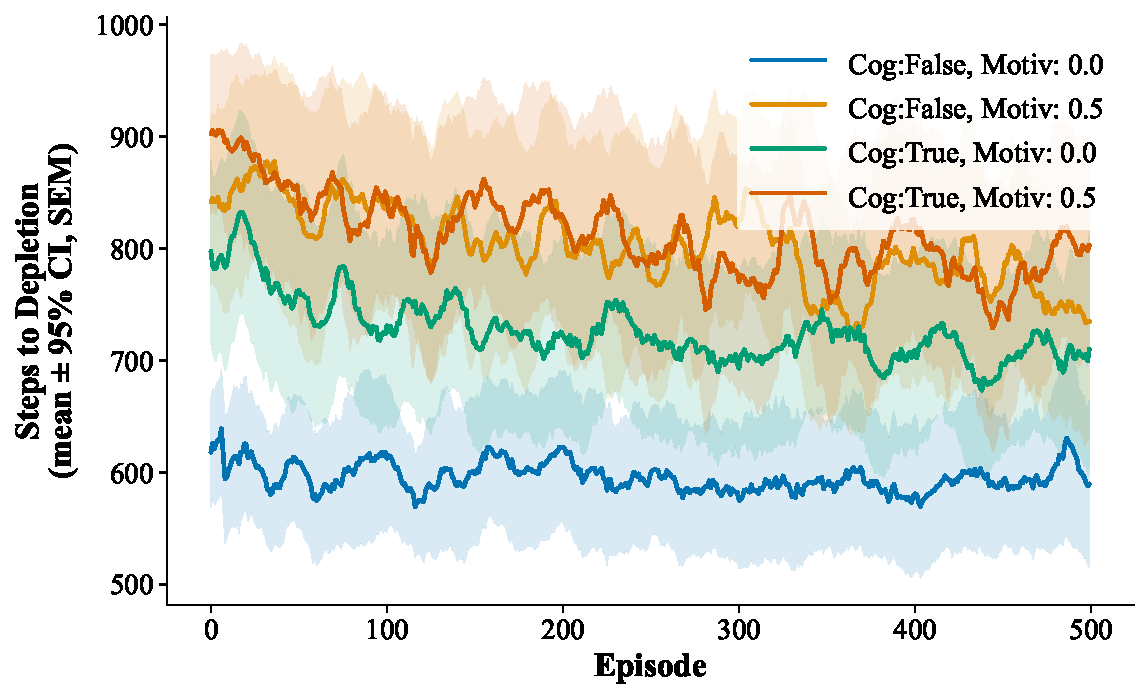
\includegraphics[width=0.8\textwidth]{figures/results/matrix_steps_trajectory}
  \caption{Episode length as a function of empathic properties across episodes. \textit{Cog}: ability to perceive others' emotions; \textit{Motiv}: empathic motivation.}
  \label{fig:matrix_steps_traj}
\end{figure}

\begin{figure}[H]
  \centering
  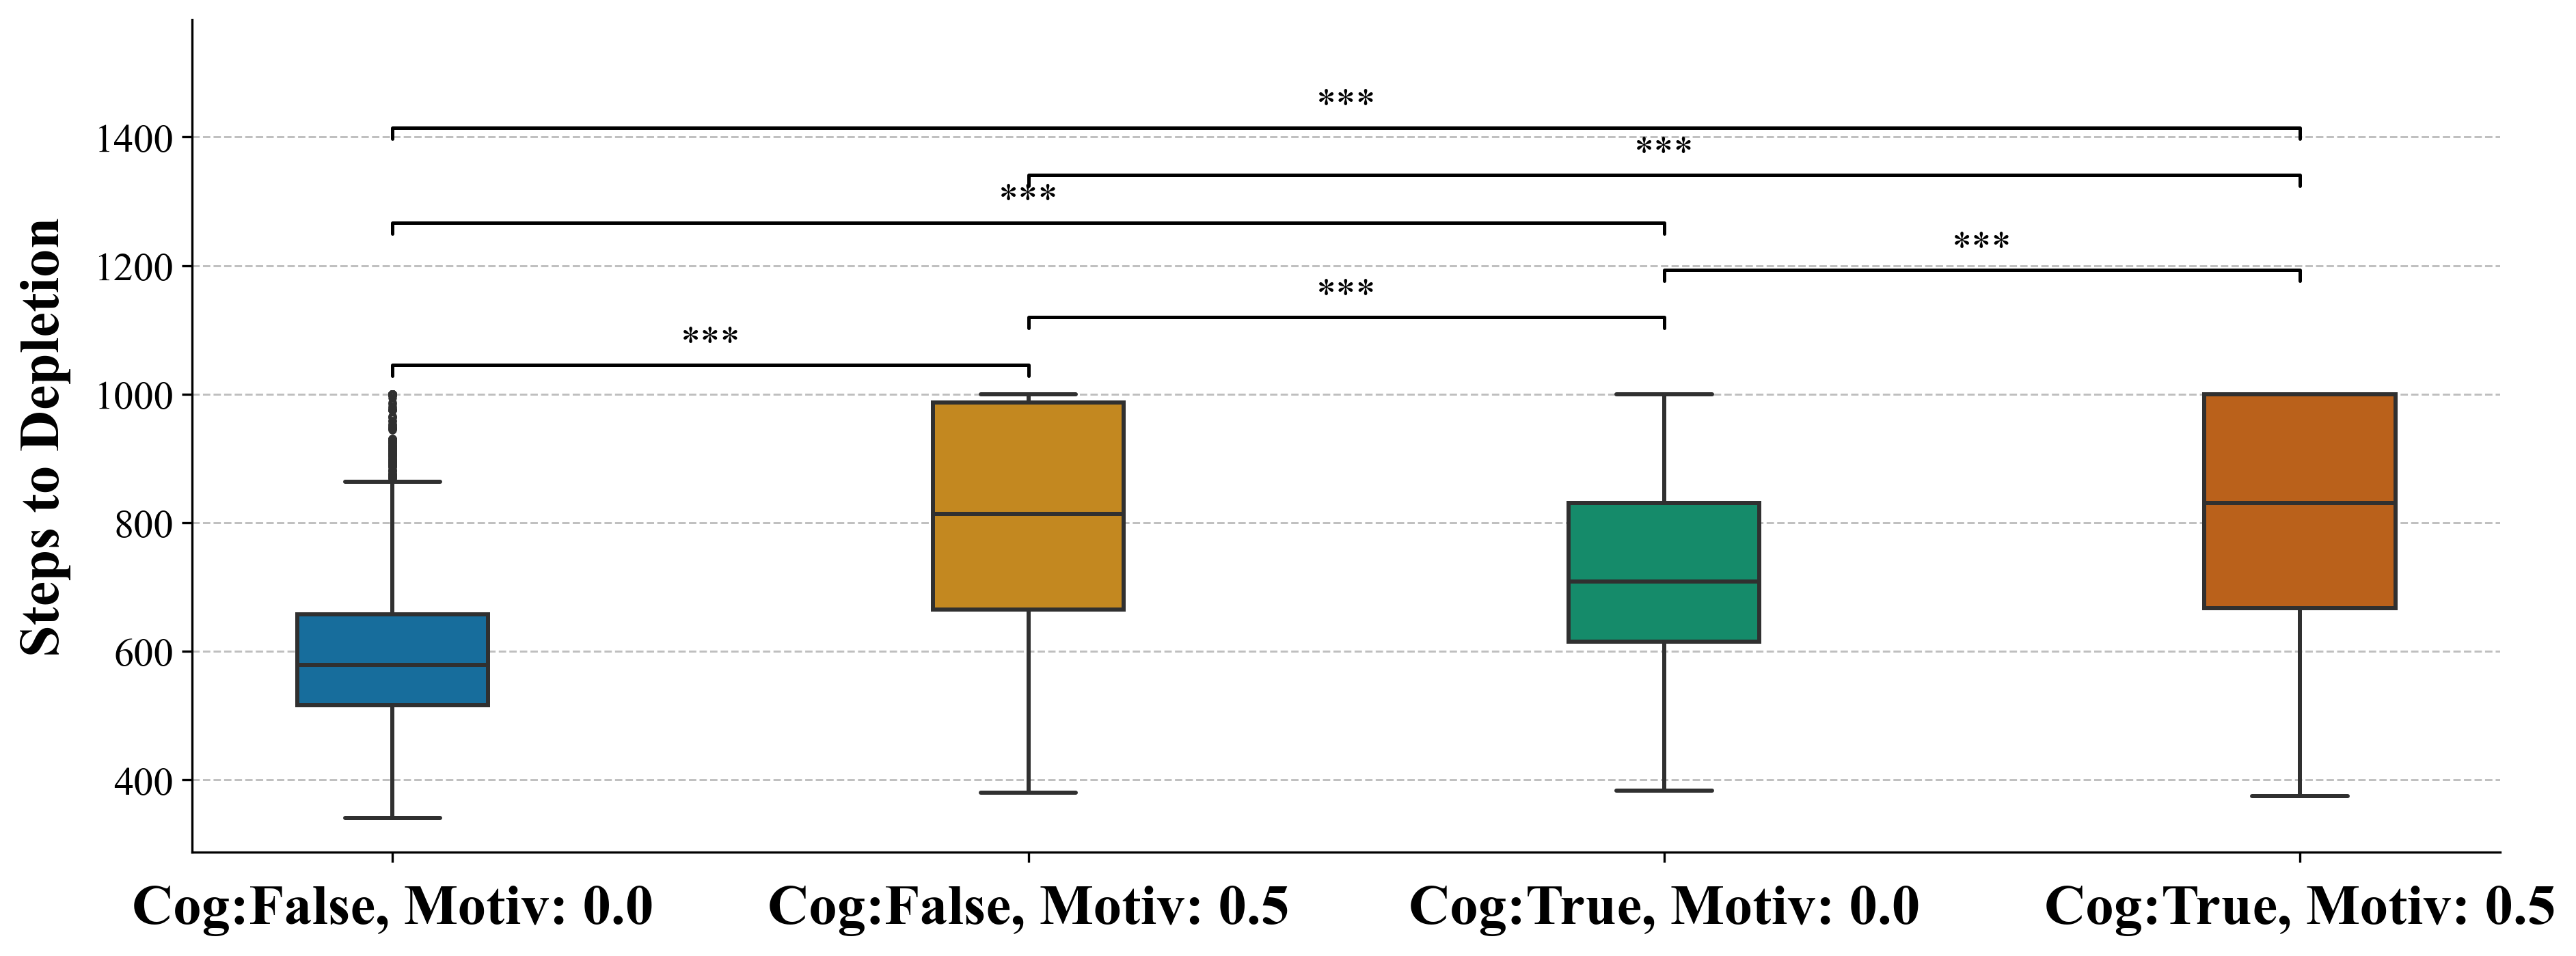
\includegraphics[width=\textwidth]{figures/results/full star matrix depletion.png}
  \caption{Episode length as a function of empathic properties, aggregated across episodes.}
  \label{fig:matrix_steps_box}
\end{figure}

A two-way ANOVA on episode length revealed significant main effects of emotion-perception ability ($F(1, 8) = 68.29$, $p < .001$, $\eta^2 = .12$) and empathic motivation ($F(1, 8) = 396.53$, $p < .001$, $\eta^2 = .72$). Specifically, simulations in which agents were able to perceive others' emotions showed greater sustainability than agents without this ability, and higher levels of empathic motivation were associated with longer episode durations. In addition, the interaction between the two factors was significant ($F(1, 8) = 75.53$, $p < .001$, $\eta^2 = .14$), indicating that the positive effect of cognitive empathy on sustainability was stronger when motivational empathy was high than when it was low. Likewise, the effect of motivational empathy was amplified when agents were able to perceive others' emotions.

\subsubsection{Gini Coefficient.}
Figure~\ref{fig:matrix_gini_traj} shows the evolution of the Gini coefficient across episodes, and Fig.~\ref{fig:matrix_gini_box} presents the aggregated distributions.

\begin{figure}[H]
  \centering
  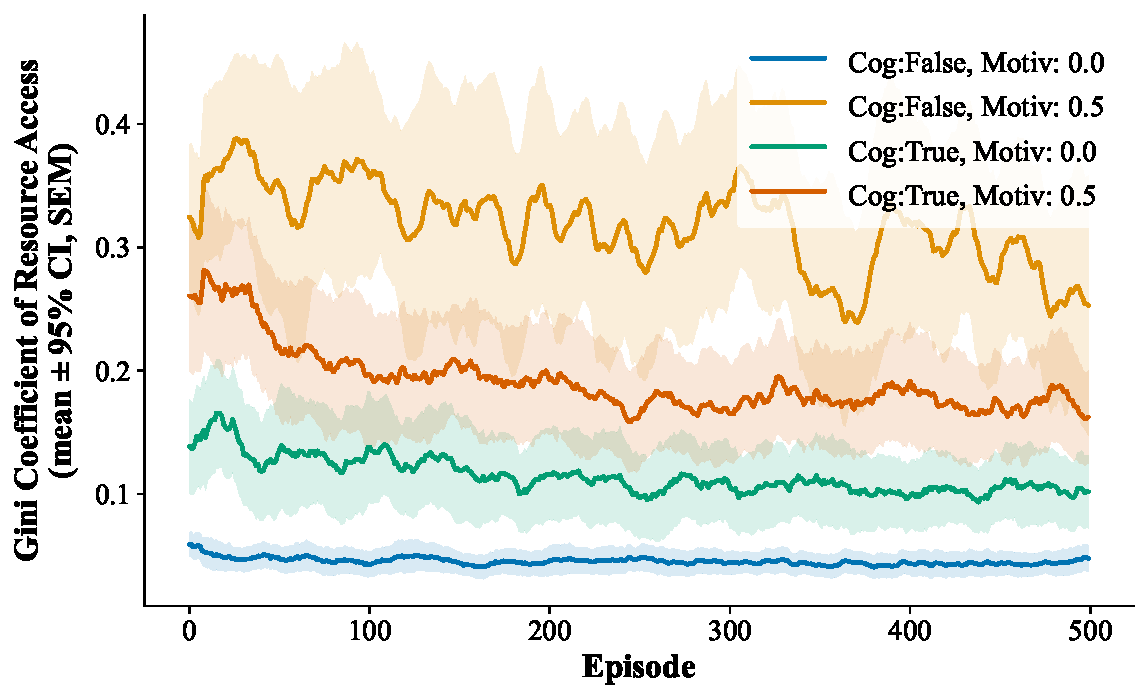
\includegraphics[width=0.8\textwidth]{figures/results/matrix_gini_trajectory.pdf}
  \caption{Fairness (Gini coefficient of resource access) as a function of empathic properties across episodes.}
  \label{fig:matrix_gini_traj}
\end{figure}

\begin{figure}[H]
  \centering
  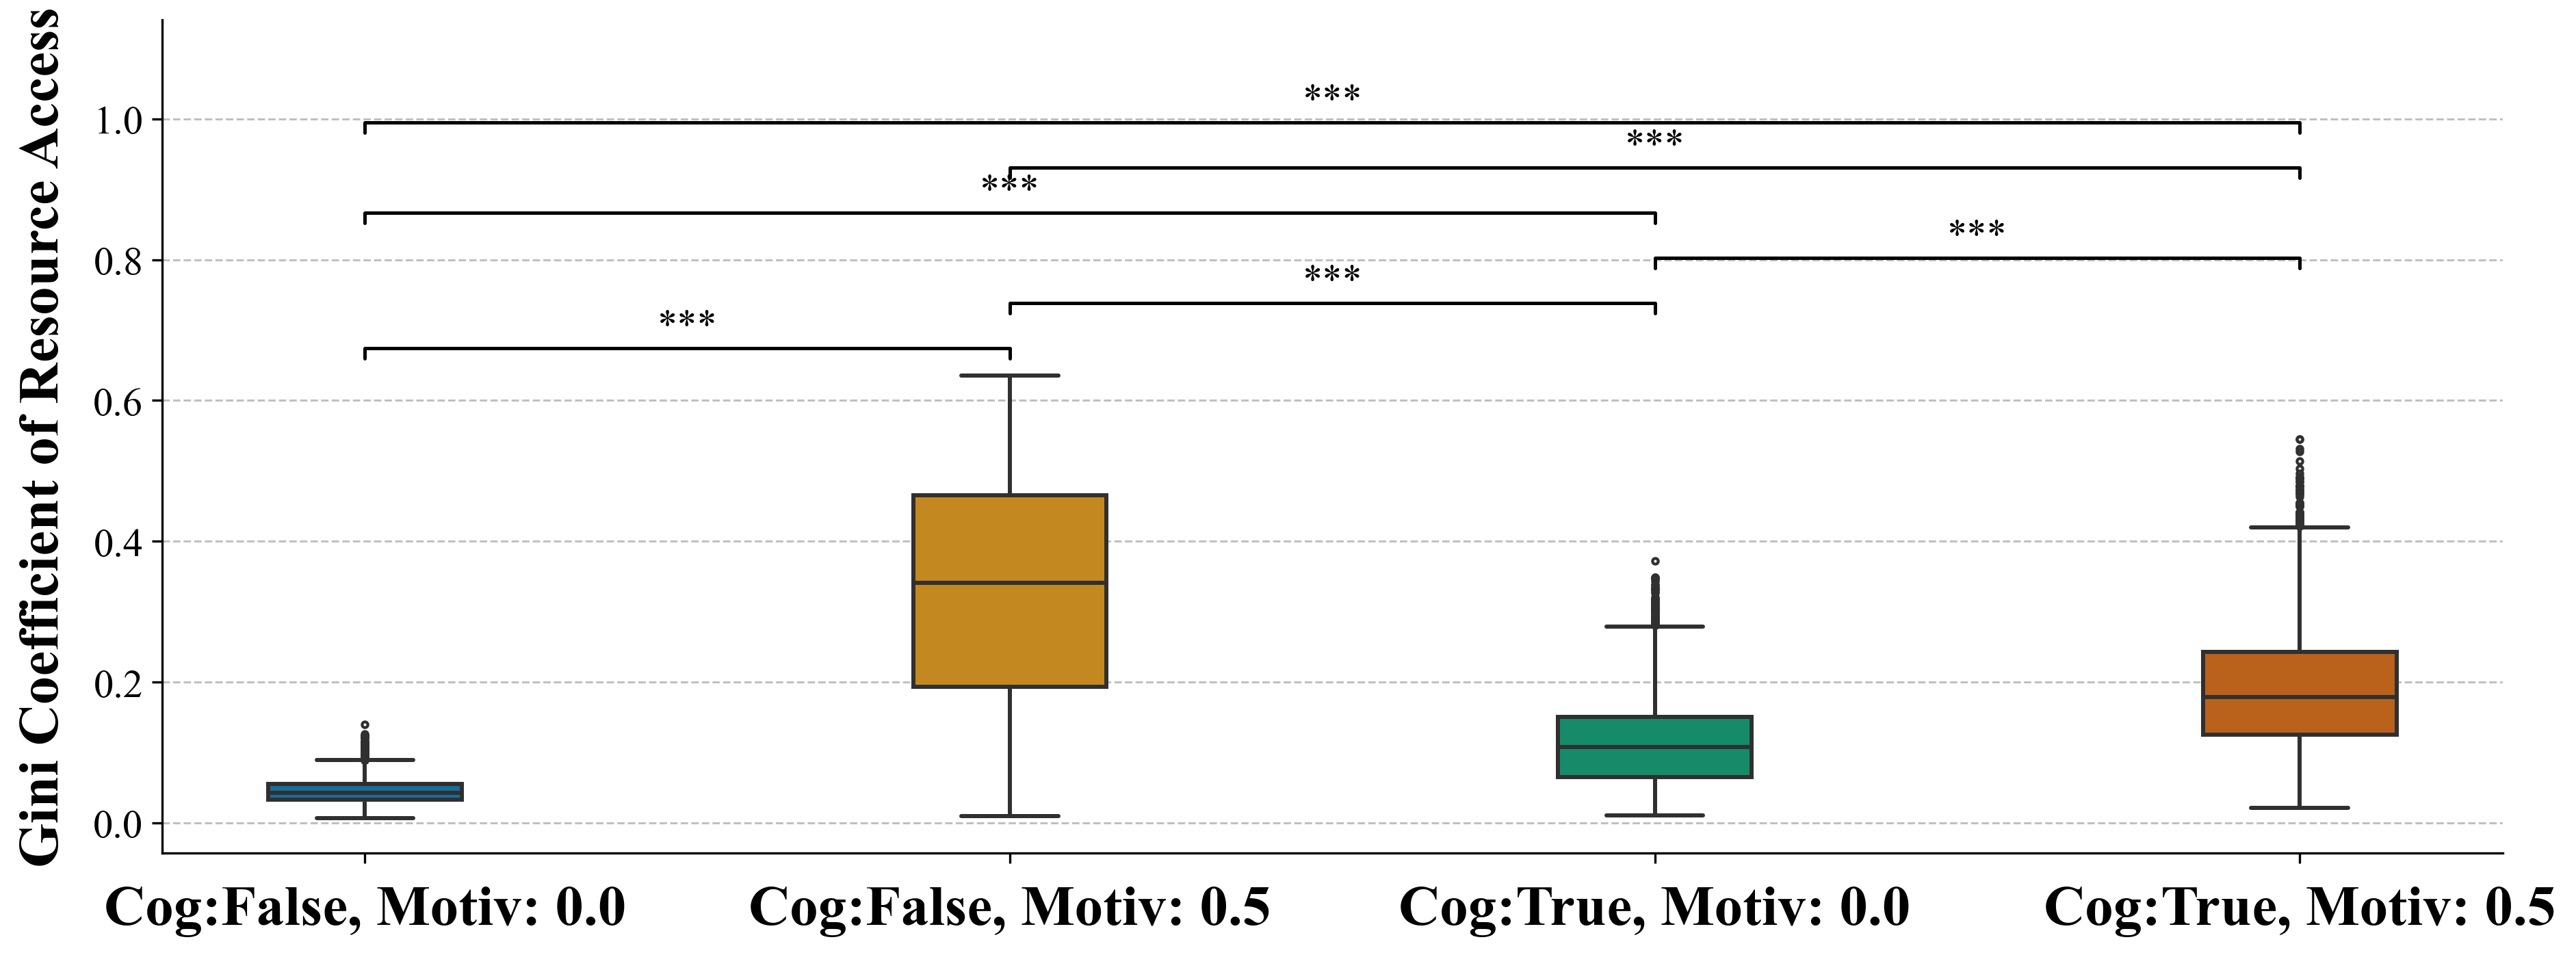
\includegraphics[width=\textwidth]{figures/results/full star matrix gini.png}
  \caption{Fairness (Gini coefficient of resource access) as a function of empathic properties, aggregated across episodes.}
  \label{fig:matrix_gini_box}
\end{figure}

A two-way ANOVA on the Gini coefficient revealed significant main effects of emotion-perception ability ($F(1, 8) = 68.29$, $p < .001$, $\eta^2 = .12$) and empathic motivation ($F(1, 8) = 396.53$, $p < .001$, $\eta^2 = .72$). Specifically, simulations where agents were able to perceive others' emotions exhibited higher inequality levels than agents without this ability, and higher levels of empathic motivation were associated with higher Gini coefficients. In addition, a significant interaction between the two factors was observed ($F(1, 8) = 75.53$, $p < .001$, $\eta^2 = .14$), indicating that the inequality associated with motivational empathy was lower when agents were able to see others' emotions was high than when it was low.

\subsection{Study 2: More Altruistic Motivation, Less Depletion}

\subsubsection{Episode Length.}
Figure~\ref{fig:alpha_steps_traj} shows the evolution of episode length across episodes for varying degrees of altruism, and Fig.~\ref{fig:alpha_steps_box} presents the aggregated distributions.

\begin{figure}[H]
  \centering
  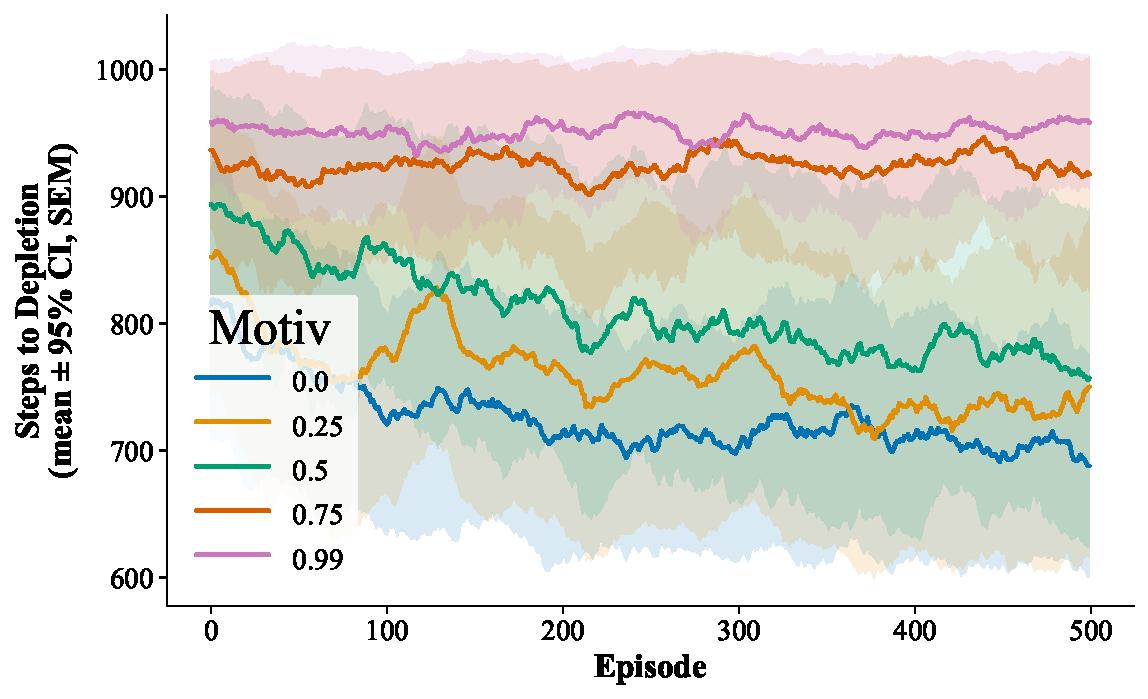
\includegraphics[width=0.8\textwidth]{figures/results/alpha_steps_trajectory}
  \caption{Episode length as a function of the degree of altruism ($\alpha$) across episodes.}
  \label{fig:alpha_steps_traj}
\end{figure}

\begin{figure}[H]
  \centering
  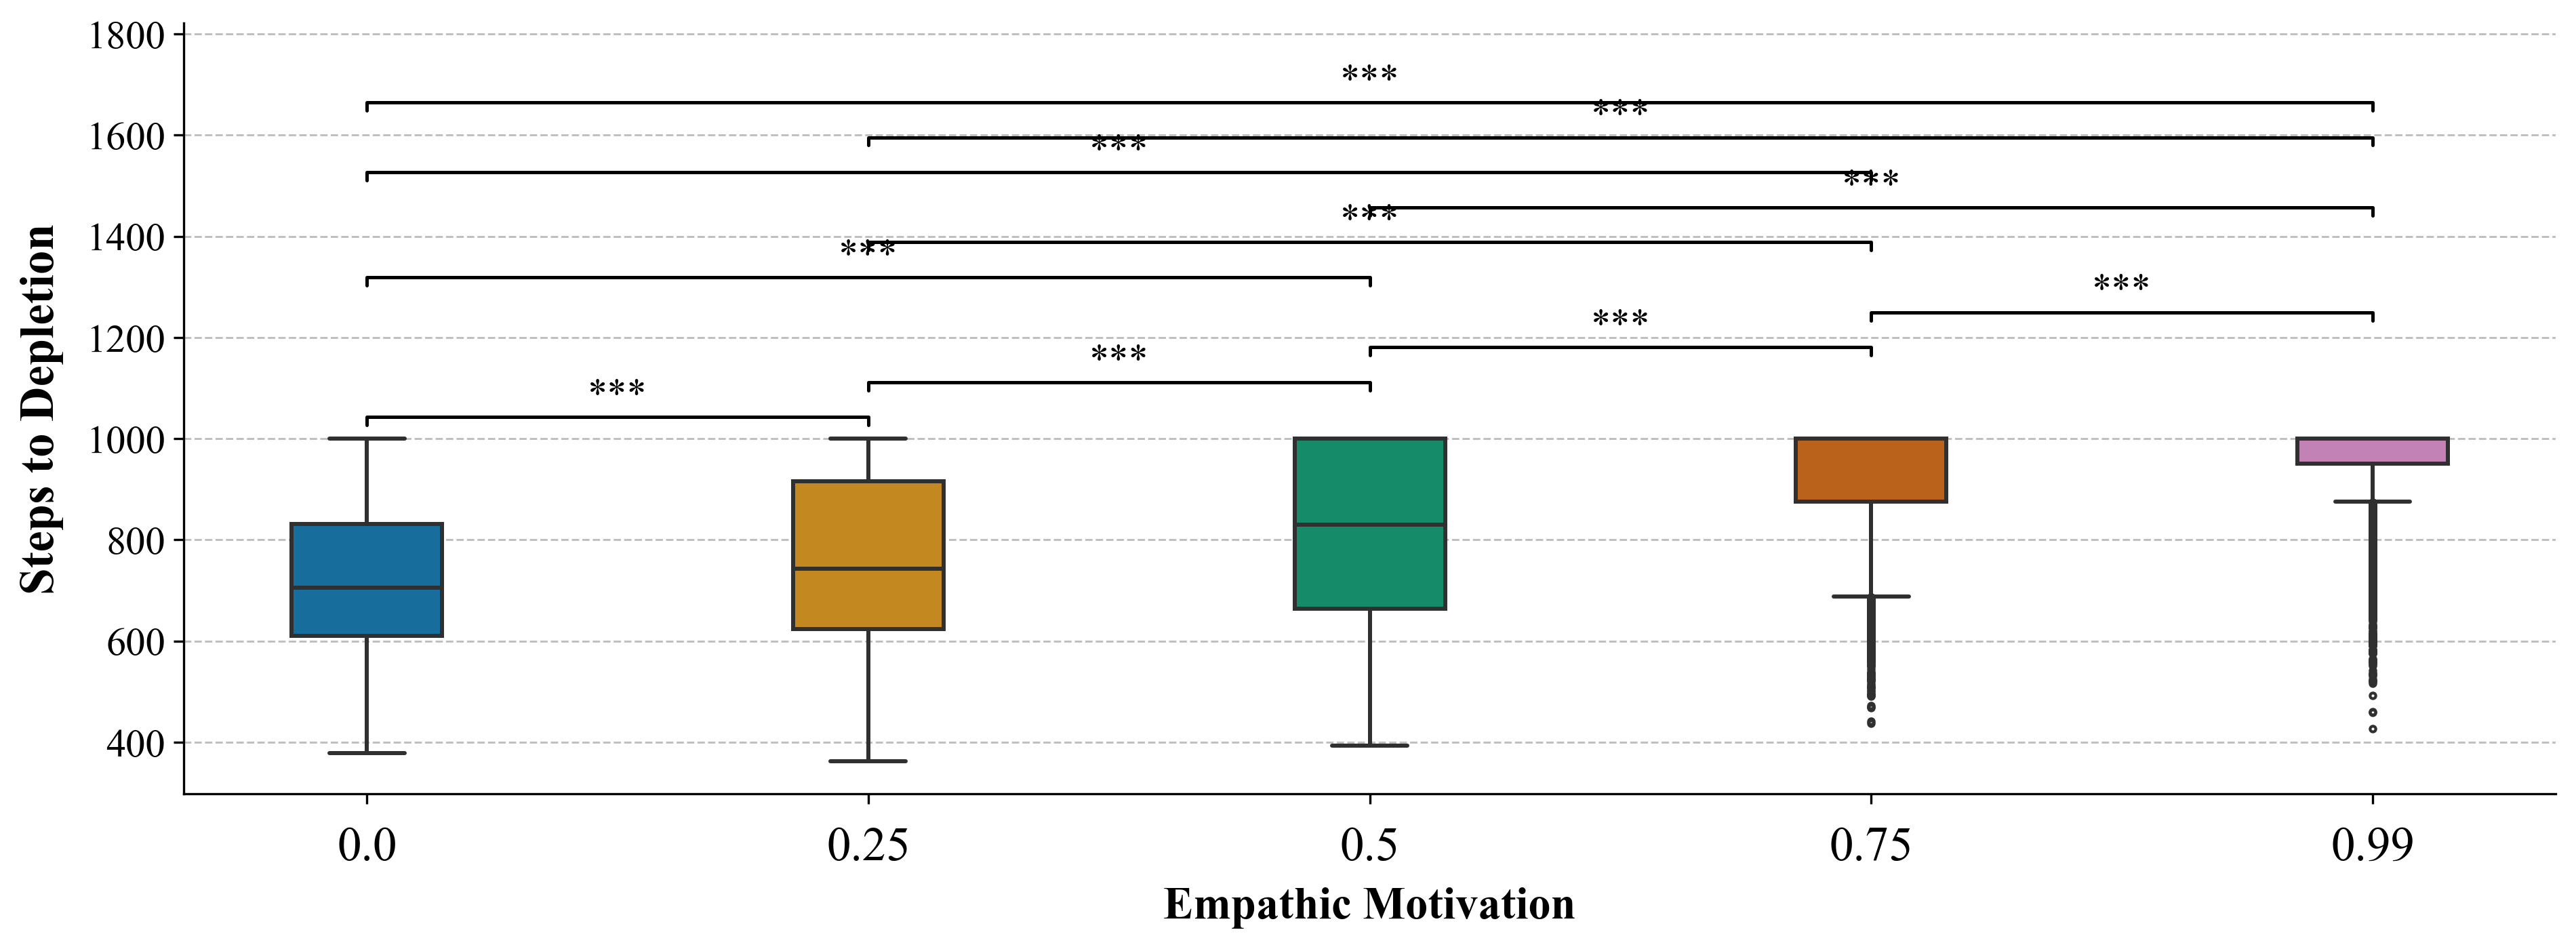
\includegraphics[width=\textwidth]{figures/results/full star alpha depletion.png}
  \caption{Episode length as a function of the degree of altruism ($\alpha$), aggregated across episodes.}
  \label{fig:alpha_steps_box}
\end{figure}

A positive Spearman correlation was found between the number of steps before depletion and the empathic motivation parameter ($r_s(22) = .92$, $p < .001$), indicating that simulations with agents that have higher levels of altruistic motivation were associated with longer-lasting episodes before depletion occurred.

\subsubsection{Gini Coefficient.}
Figure~\ref{fig:alpha_gini_traj} shows the evolution of the Gini coefficient across episodes, and Fig.~\ref{fig:alpha_gini_box} presents the aggregated distributions.

\begin{figure}[H]
  \centering
  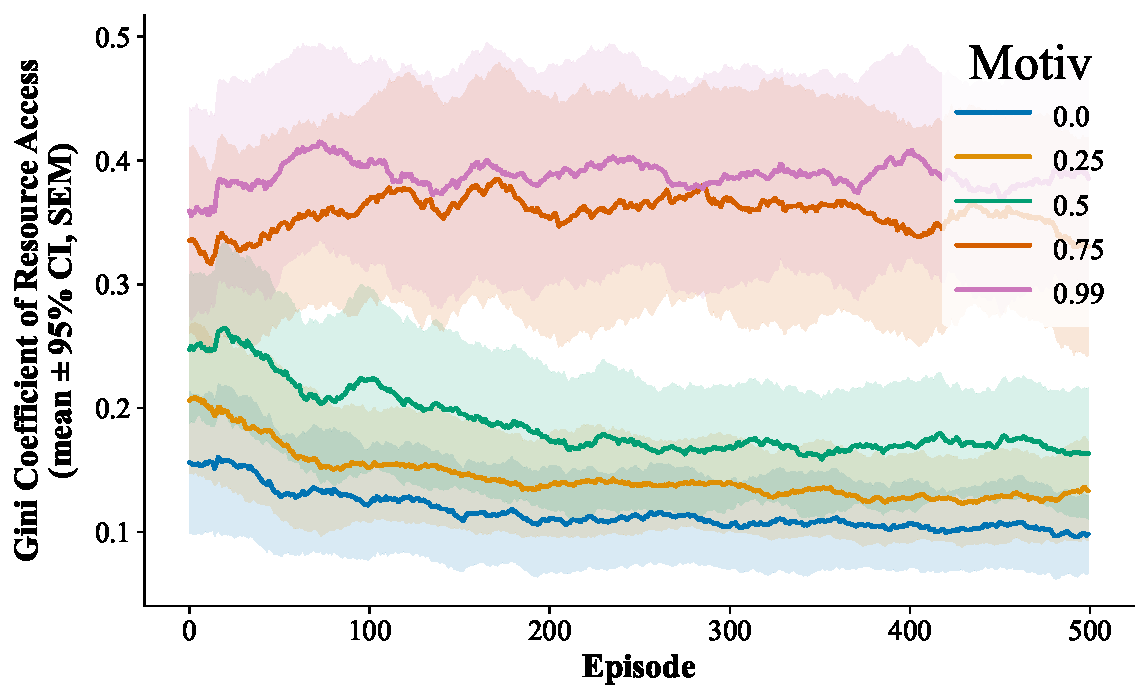
\includegraphics[width=0.8\textwidth]{figures/results/alpha_gini_trajectory}
  \caption{Fairness (Gini coefficient of resource access) as a function of the degree of altruism ($\alpha$) across episodes.}
  \label{fig:alpha_gini_traj}
\end{figure}

\begin{figure}[H]
  \centering
  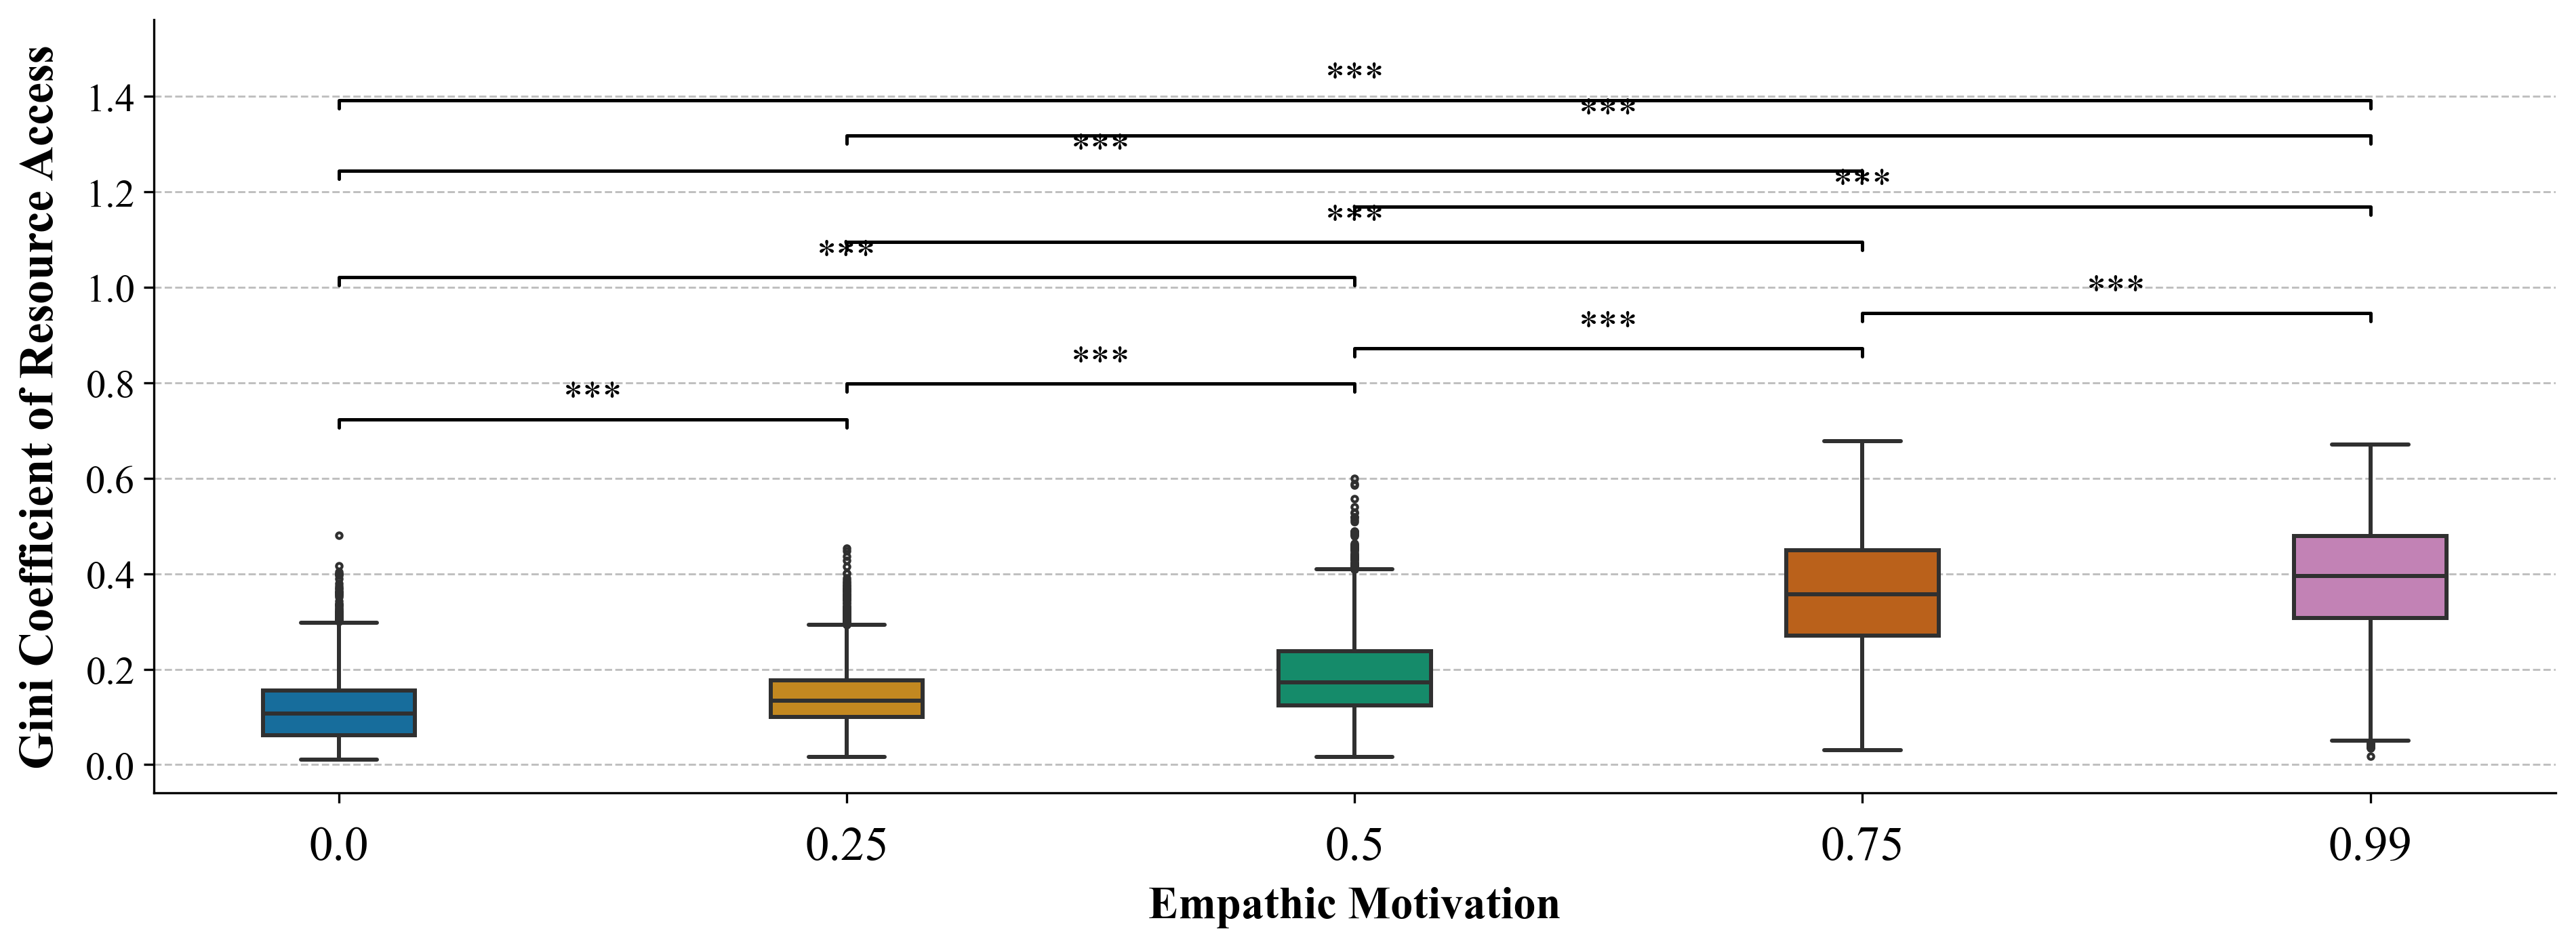
\includegraphics[width=\textwidth]{figures/results/full star alpha Gini.png}
  \caption{Fairness (Gini coefficient of resource access) as a function of the degree of altruism ($\alpha$), aggregated across episodes.}
  \label{fig:alpha_gini_box}
\end{figure}

A positive Spearman correlation was found between fairness and the empathic motivation parameter ($r_s(22) = .96$, $p < .001$), indicating that simulations with agents that have higher levels of altruistic motivation were associated with less equitable resource distribution.
